%\chapter{det-comp}


%%%%%%%%%%%%%%%%%%%%%%%%%%%%%%%%%%%%%%%%%%%%%%
%\section{Anode Plane Assemblies}

%%%%%%%%%%%%%%%%%%%%%%%%%%%%%%%%%%%%%%%%%%%%%%
%\section{Cathode Plane Assemblies}

%%%%%%%%%%%%%%%%%%%%%%%%%%%%%%%%%%%%%%%%%%%%%%
%\section{Field Cage}

%%%%%%%%%%%%%%%%%%%%%%%%%%%%%%%%%%%%%%%%%%%%%%
\section{TPC high-voltage (HV) components}

%%%%%%%%%%%%%%%%%%%%%%%%
\subsection{Scope and requirements}

The TPC high voltage (HV) components include the HV power supply, cables,
filter circuit, HV feedthrough,  and monitoring for currents and voltages (both steady
state and transient).

A schematic of the complete TPC HV circuit is shown in Figure~\ref{fig:TPCHVcircuit}.

\begin{cdrfigure}[TPC HV circuit]{TPCHVcircuit}{A schematic of the TPC high voltage circuit.}
  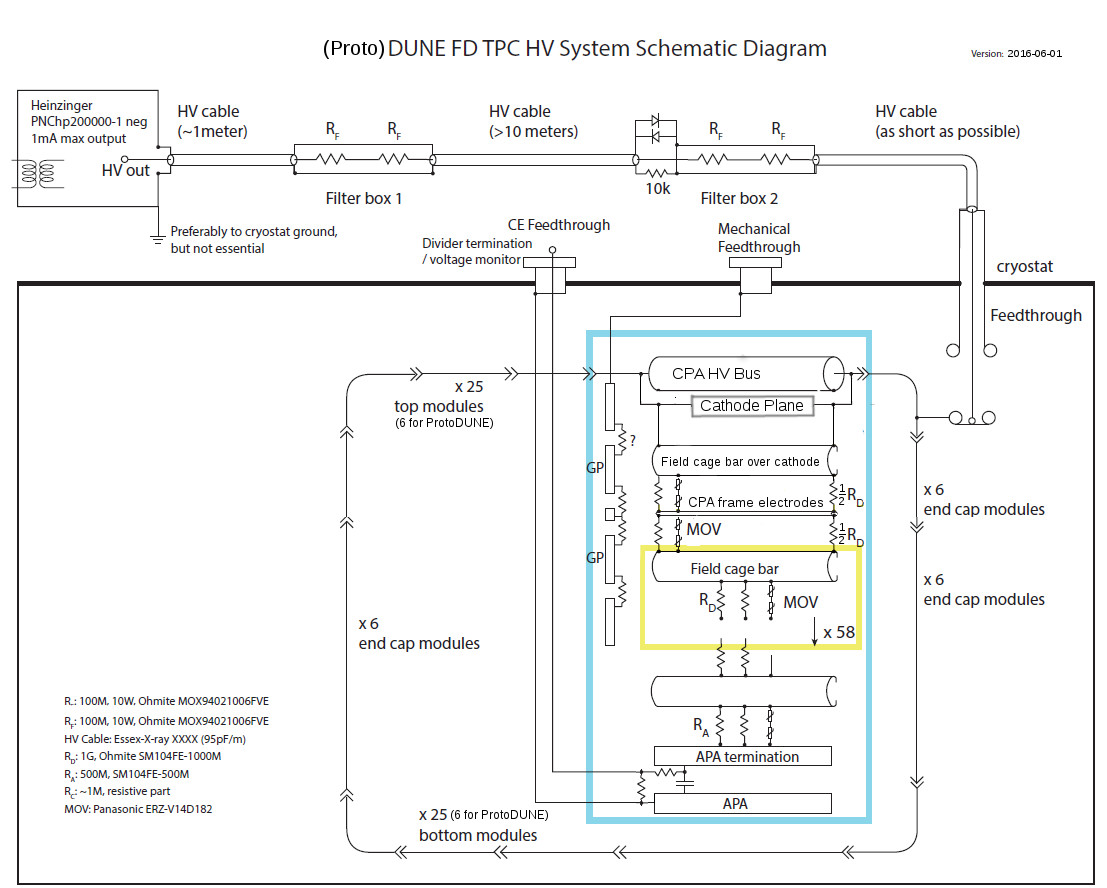
\includegraphics[width=0.95\textwidth]{VR_TPC_HV_schem-mod-1}
\end{cdrfigure}

The cathode plane is biased at \SI{-180}{kV} to provide the
required \SI{500}{V/cm} drift field.  It is 
powered by a dedicated HV power supply through an RC filter and HV 
feedthrough.  The power supply for the cathode plane must be able
to provide \SI{-200}{kV}.  The output voltage
ripple must not introduce more than 10\% 
of the equivalent thermal
noise from the front-end electronics. The power supply must be
programmable to shut down its output at a certain current
limit. During power cycling, both controlled and uncontrolled, the voltage 
ramp rate at the feedthrough must be limited
to prevent damage to the in-vessel electronics from excess charge
injection. The HV feedthrough must be able to withstand \SI{-250}{kV}
in its center conductors in a \SI{1}{atm} argon gas environment when
terminated in liquid argon.


%%%%%%%%%%%%%%%%%%%%%%%%
\subsection{HV feedthrough design, power supply and cabling}
%In the present baseline option, 
The design of the HV feedthrough as well as the procurement of the HV power supply, cables, and possibly filter
circuits, are activities being jointly pursued by the \pdsp and ProtoDUNE-DP efforts. In particular:

\begin{itemize}	
\item The Heinzinger 300-kV power supply (residual ripple less than $10^{-5}$) and cable specified for ProtoDUNE-DP  are  well suited for \pdsp, which operates at a lower HV setting.
\item The present ProtoDUNE-DP HV feedthrough design is adaptable to \pdsp without any major modification in its dimensions or mechanical features.
\item The filtering scheme and the monitoring system required for \pdsp is more demanding than that for ProtoDUNE-DP, due to its more sensitive front-end electronics, and can be used for both detectors.
\item Common spare components are also being utilized.
\end{itemize}

The %present 
design of the 300-kV feedthrough is based on the very successful construction technique adopted for the ICARUS HV feedthrough, which was operated at 75\,kV without interruption for more than three years without any failure. The feedthrough was also successfully operated for several days as a test after the run at 150\,kV.  
%A coaxial geometry is adopted: 
The design is based on a coaxial geometry, with an inner conductor (HV) and an outer conductor (ground) insulated by ultra-high-molecular-weight polyethylene (UHMW PE)  as shown in Figure~\ref{fig:hv-feed-through}. 

The outer conductor, made of a stainless-steel tube, surrounds the insulator, extending down through the cryostat into the LAr. 
In this geometry, the electric field is %always 
confined within regions occupied by high-dielectric-strength media (UHMW PE and LAr).  The inner conductor is made of a thin-walled stainless steel tube to minimize the heat input and to avoid the creation of argon gas bubbles around the lower end of the feedthrough. A contact, welded at the upper end for the
connection to the HV cable, and a round-shaped elastic contact for the connection to the cathode, screwed at the lower end, completes the inner electrode. Special care has been taken in the assembly to ensure complete filling  of the space between the inner and outer conductors with the PE dielectric, and to guarantee leak-tightness at ultra-high vacuum levels.


\begin{cdrfigure}[HV feedthrough]{hv-feed-through}{Preliminary design of the HV feedthrough.}
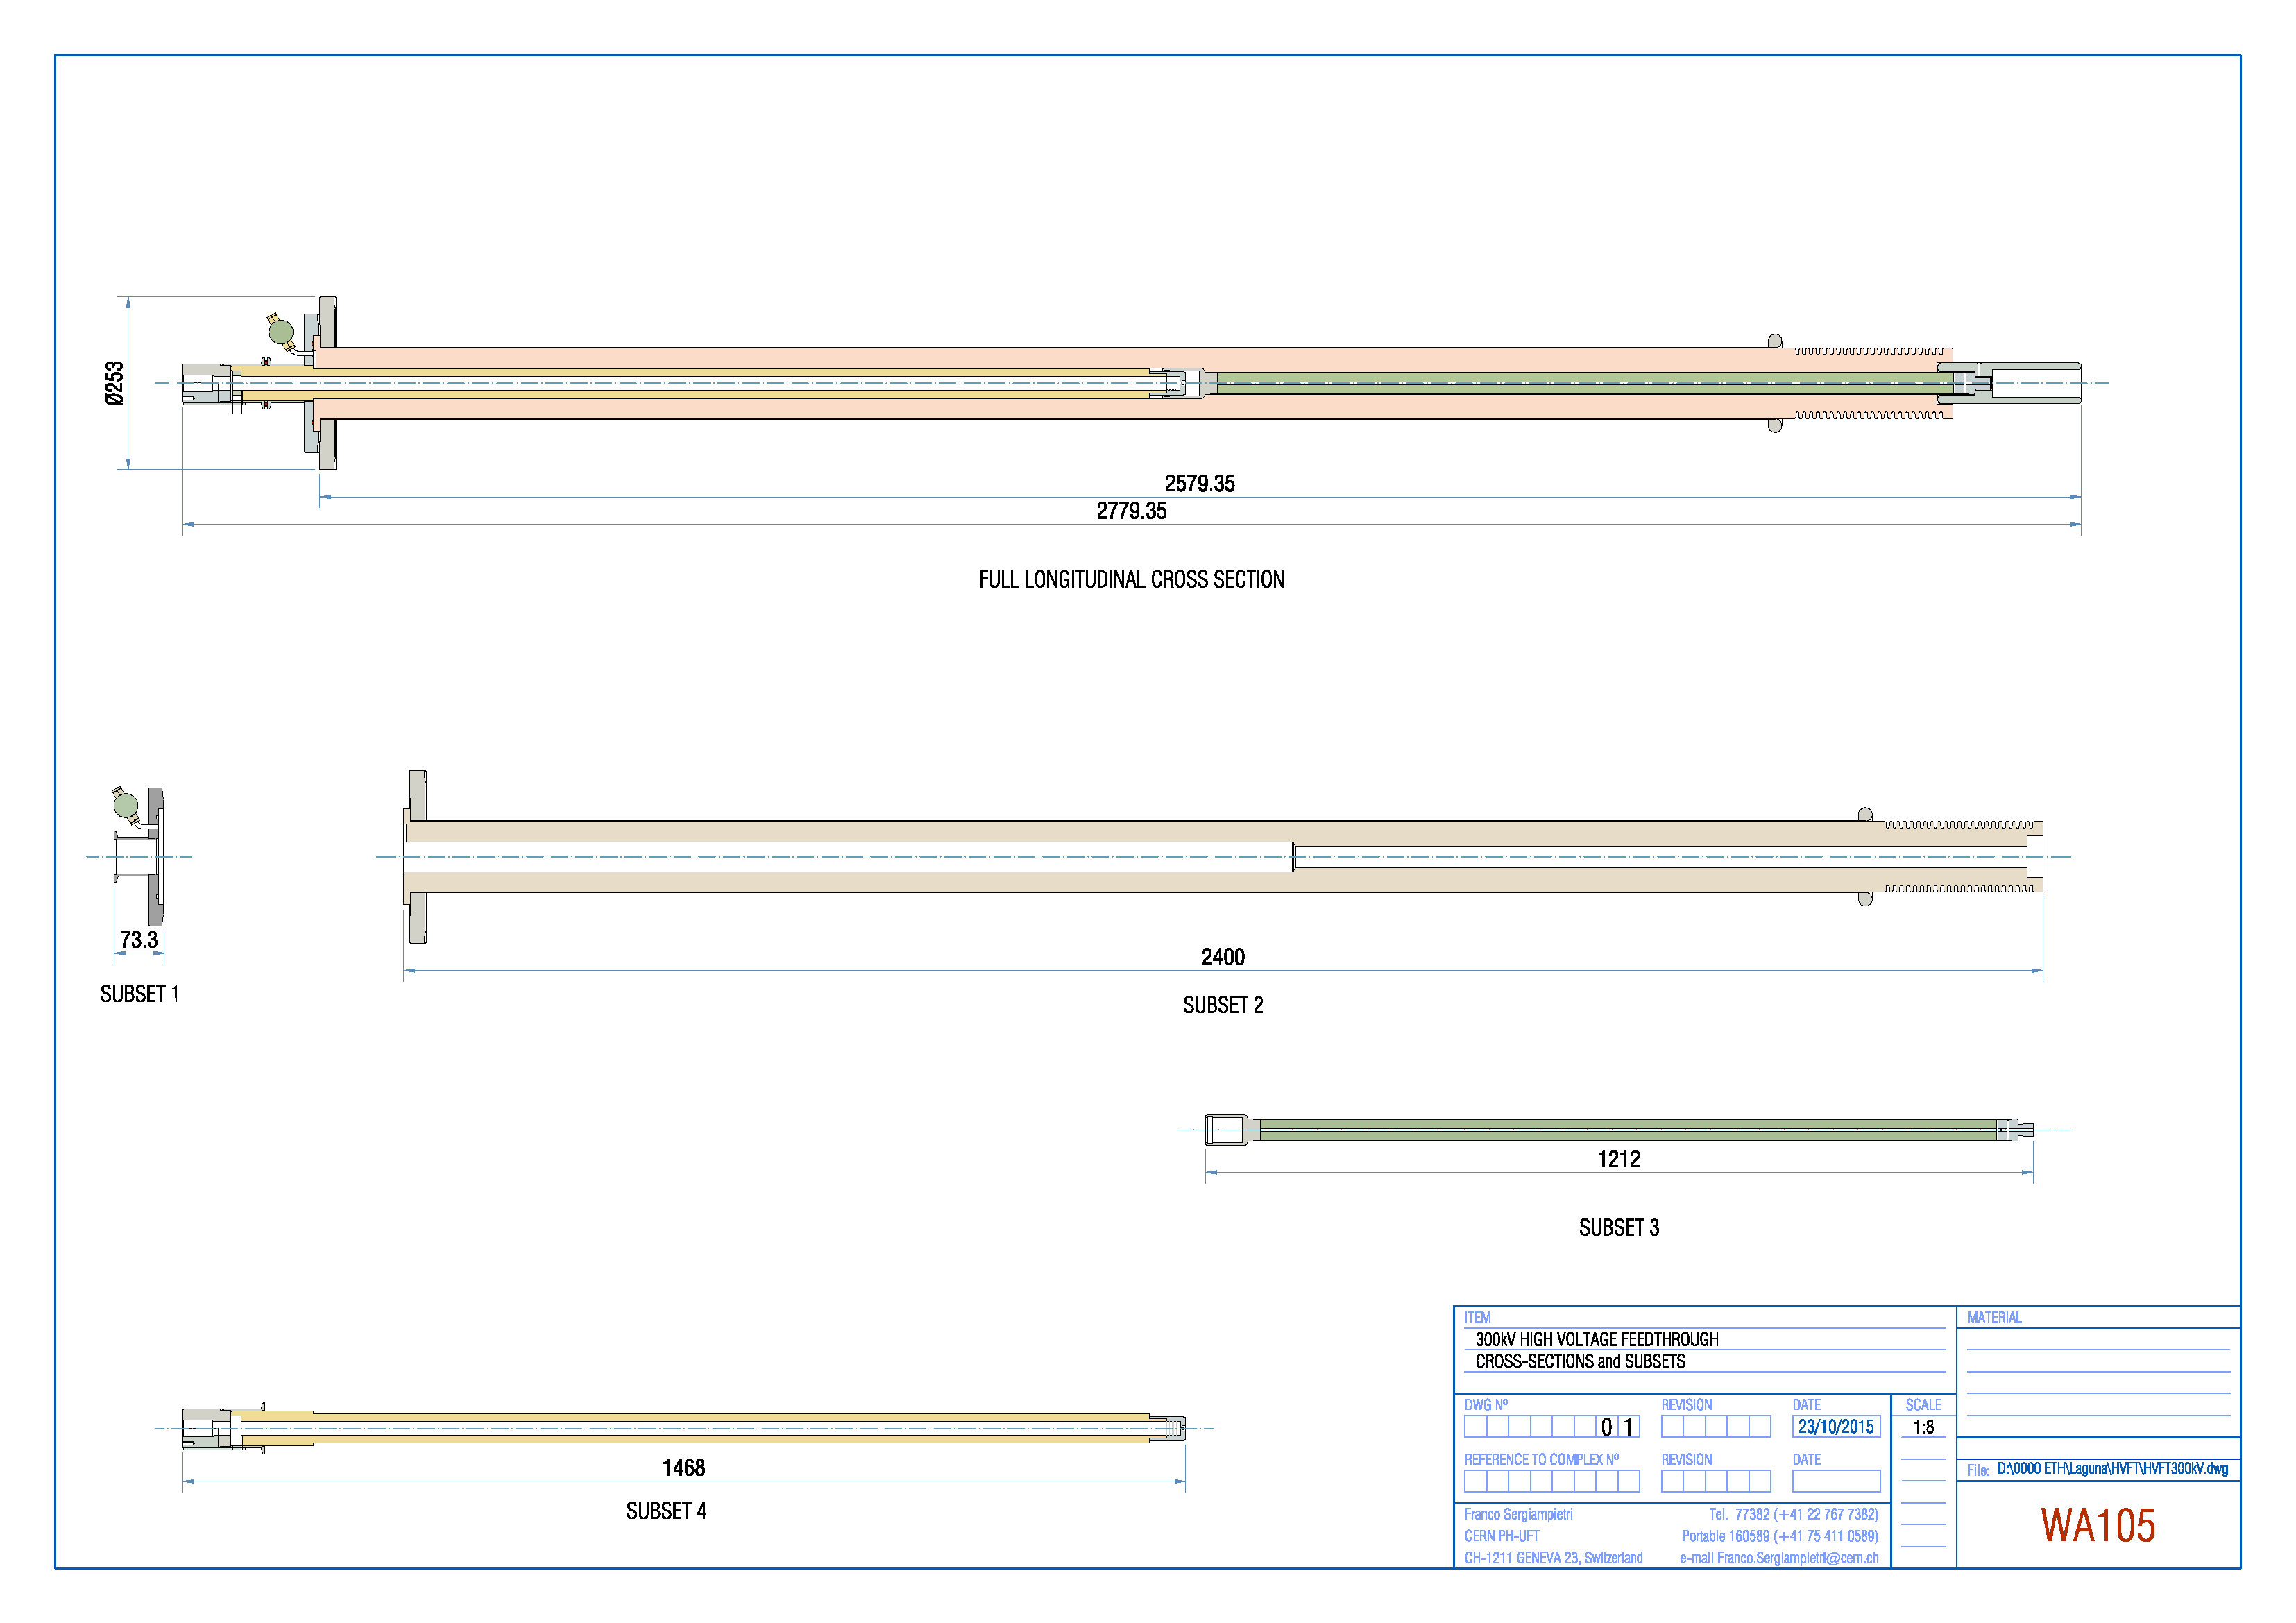
\includegraphics[width=0.95\textwidth]{tpc_HVFT300kV-1.png}
\end{cdrfigure}





%%%%%%%%%%%%%%%%%%%%%%%%
\subsection{HV monitoring}

HV-circuit monitoring devices include a toroid transformer to detect
spikes and noise in the current draw, and a monitoring point at the end
of the field cage resistor chain, which also provides a means to
control field-shaping around the edge of the
APA.

